\documentclass[a4paper, 12pt]{article}

\usepackage[top=2cm, bottom=2cm, left=2.5cm, right=2.5cm]{geometry}
\usepackage[utf8]{inputenc}
\usepackage{array}
\usepackage{graphicx}

\graphicspath{{img/}}

\begin{document}
\begin{flushleft}
\includegraphics{logo}\\
\textbf{UNIVERSIDADE ESTADUAL DE PONTA GROSSA} \\
SISTEMA UNIVERSIDADE ABERTA DO BRASIL - UAB \\
\underline{Licenciatura em Matemática | Polo UAB em Jacarezinho}\end{flushleft} 
\textbf{ALUNO:} Ricardo Medeiros da Costa Junior   \textbf{RA:} 151774301 \\
\textbf{DISCIPLINA:} 101505 - Cálculo Diferencial e Integral II \\
\textbf{ATIVIDADE:} Tarefa - Unidade III (Valor: 6 pontos) \\
\textbf{TUTOR(A):} Adilane de Assis Ferreira \\
\textbf{PERÍODO:} Quarto Período \\
\begin{enumerate}
\item ({\it Valor: 1,0 ponto}) Calcule a área abaixo do gráfico da função $ f(x)= x^{3} $, sob o intervalo $ [0,b] $
%  \begin{figure}[h!]
%  \centering
%  
\includegraphics[width=0.7\textwidth]{1}
%  \end{figure}

  \begin{figure}[h!]
  \centering
  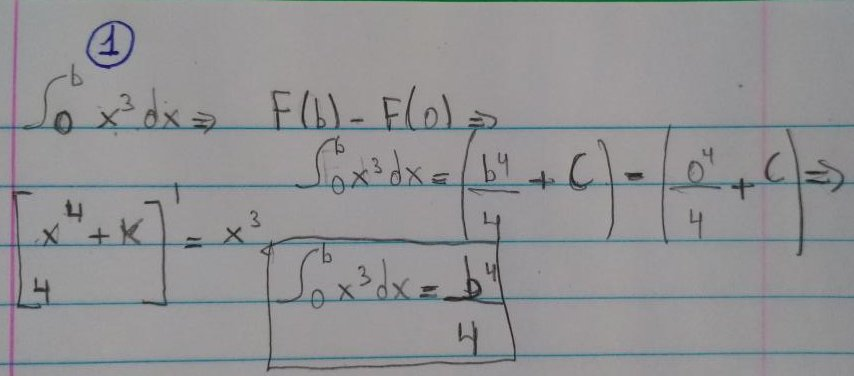
\includegraphics[width=0.7\textwidth]{resp1}
  \end{figure} \newpage

  \item ({\it Valor: 0,5 pontos cada}) Calcule as seguintes integrais definidas:
  \begin{description}
  \item[a.] $ \int_0^{1}x(\sqrt{x}+\sqrt[3]{x})dx $

  \begin{figure}[h!]
  \centering
  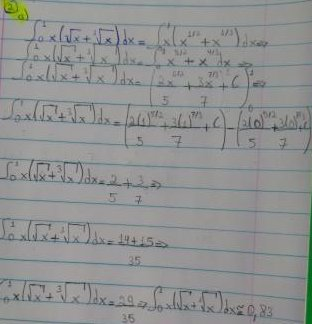
\includegraphics[width=0.7\textwidth]{resp2a}
  \end{figure} \newpage 
    
  \item[b.] $ \int_0^{1}xe^{x^{2}}dx $
  \begin{figure}[h!]
  \centering
  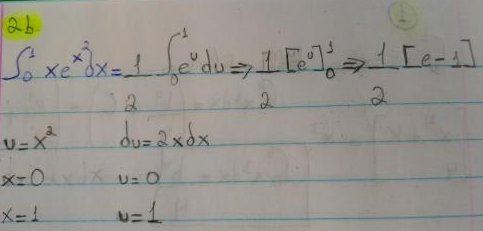
\includegraphics[width=0.7\textwidth]{resp2b}
  \end{figure}  \newpage
  
  \item[c.] $ \int_0^{1}e^{2x}\sqrt{e^{2x}+1}dx $
  \begin{figure}[h!]
  \centering
  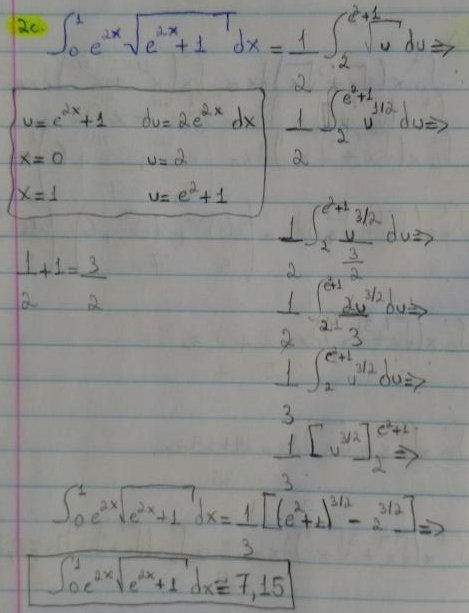
\includegraphics[width=0.7\textwidth]{resp2c}
  \end{figure} \newpage
  
  \item[d.] $ \int_0^{\pi}x[sen(x)+cos(x)]dx $
  \begin{figure}[h!]
  \centering
  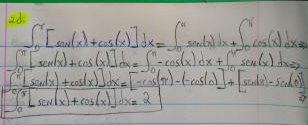
\includegraphics[width=0.7\textwidth]{resp2d}
  \end{figure}  \newpage
  
  \end{description}
\item ({\it Valor: 1,0 ponto}) A curva $ y = x^{3} - 9x $ tem um arco acima do eixo \emph{x}. Calcule a área da região sob o gráfico.
%\begin{figure}[h!]
%  \centering
%  
\includegraphics[width=0.7\textwidth]{3}
%\end{figure}  
  
\item ({\it Valor: 1,0 ponto}) Calcule a área limitada pela curva $ y = 2x + \frac{1}{x^{2}} $, o eixo \emph{x} e as retas $ x = 1 $ e $ x = 3$.
%\begin{figure}[h!]
%  \centering
%  
\includegraphics[width=0.7\textwidth]{4}
%\end{figure} 
  
\item ({\it Valor: 1,0 ponto}) Determine a área, no primeiro quadrante, limitada por $ y = sec^{2}(x) $, $ y = 8cos(x) $ e o eixo \emph{y}.
%\begin{figure}[h!]
%  \centering
%  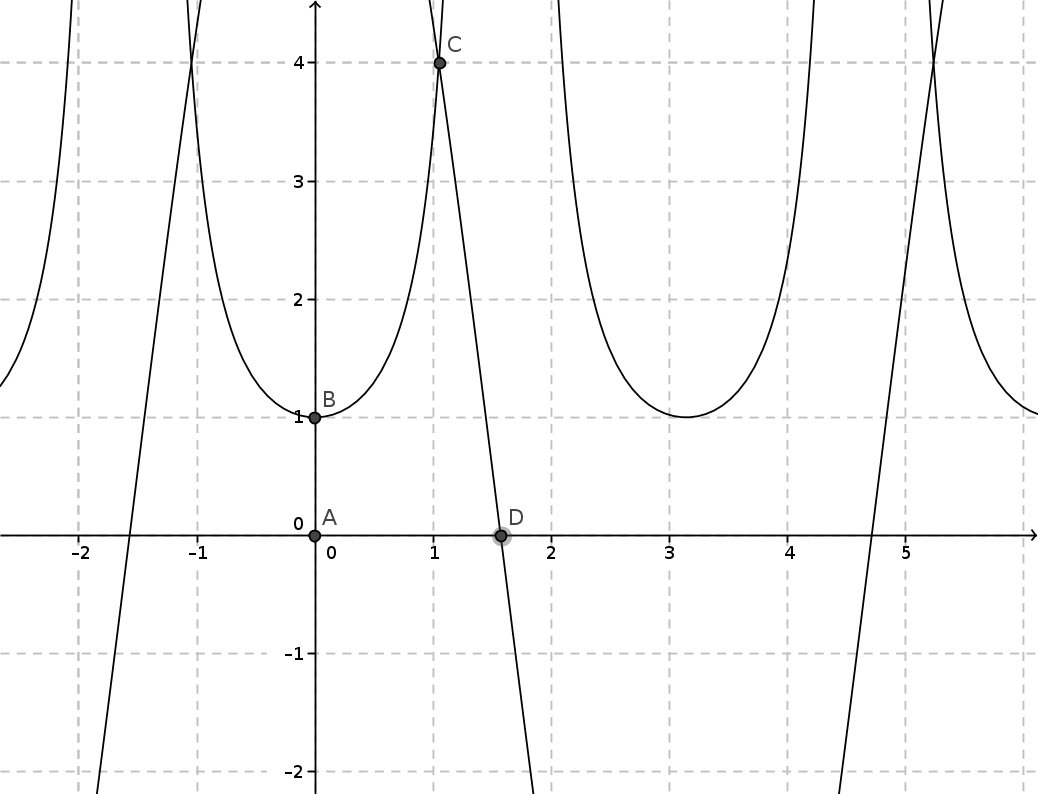
\includegraphics[width=0.7\textwidth]{5}
%\end{figure} 
  
\end{enumerate}
\end{document}
